\documentclass[10pt,aspectratio=169]{beamer}

\usetheme{Madrid}
\usepackage[T1]{fontenc}
\usepackage{tikz}
\usetikzlibrary{arrows.meta,positioning,overlay-beamer-styles}

% --- Emphasis in the theme's blue instead of the default red ---
\setbeamercolor{alerted text}{use=structure,fg=structure.fg}

% --- Give each \section its own title slide (as metropolis did) ---
\AtBeginSection[]{
  \begin{frame}
    \sectionpage
  \end{frame}
}

% --- Numbered [1], [2], ... markers for \cite and the References list ---
\setbeamertemplate{bibliography item}{\insertbiblabel}
\setbeameroption{hide notes}

\title{Signed, Sealed, Supersingular}
\subtitle{Post-quantum signatures and the Supersingular Isogeny Path Problem}
\author{Owen Waldron}
\institute{UW PMC S26 SASMS 2}
\date{\today}

\begin{document}

% ===== 1. TITLE =====
{
\setbeamertemplate{footline}{}
\begin{frame}[plain]
  \titlepage
\end{frame}
}

% ===== 2. ROADMAP =====
\begin{frame}{Outline and Goals}
  \begin{enumerate}
    \item What a \alert{digital signature} even is
    \item An important hard problem: the \alert{Supersingular Isogeny Path Problem}
    \item Why we believe that problem is \alert{hard}
    \item How you build a signature on top of it 
  \end{enumerate}
  \vspace{1em}
  \centering\small Goal: a taste for the fun math underpinning post-quantum crypto!
\end{frame}

% ===== SECTION: SIGNATURES =====
\section{What is a digital signature?}

% ===== 3. WHAT IS A DIGITAL SIGNATURE =====
\begin{frame}{The Digital Signature algorithms}
  \begin{itemize}[<+(1)->]
    \item \textbf{KeyGen}$()\to sk, pk$ \hfill {Generate a public/private key pair}
    \item \textbf{Sign}$(sk, m)\to \sigma$ \hfill use private key to sign messages
    \item \textbf{Verify}$(pk, m, \sigma)\to \{0,1\}$ \hfill anyone can verify a signature using the public key
  \end{itemize}
  \vspace{1.0em}
  \onslide<+(1)->{This is an essential primitive for verifying the source of messages.
  For example, when you visit google.ca, you want to verify that the HTML response you get was in fact delivered by Google.}
  \vspace{1.0em}
  \onslide<+(1)->{
  \begin{itemize}[<+(1)->]
    \item \textcolor{red}{\textbf{Forge}}$(pk, m)\to \sigma$ \hfill an antagonist, \emph{without} the secret key
  \end{itemize}}
  \vspace{1.0em}
  \onslide<+(1)->{
  \begin{alertblock}{}
    Signing and verifying are \textbf{easy} (fast). Forging a signature for \textit{any message} must be \textbf{hard} (slow).
  \end{alertblock}}

\end{frame}

% ===== 4. THE SECURITY RECIPE =====
\begin{frame}{How do we trust a Digital Signature scheme?}
  We can show that \textbf{forging reduces to solving a hard problem} with polynomial-time reductions.\\
  Break the signature $\;\Rightarrow\;$ you broke the problem.
  \begin{center}
    % Plain figure on click 1; swaps to the annotated version on click 2.
    % Handout keeps only the annotated version.
    \only<1|handout:0>{
      \vspace{1em}
      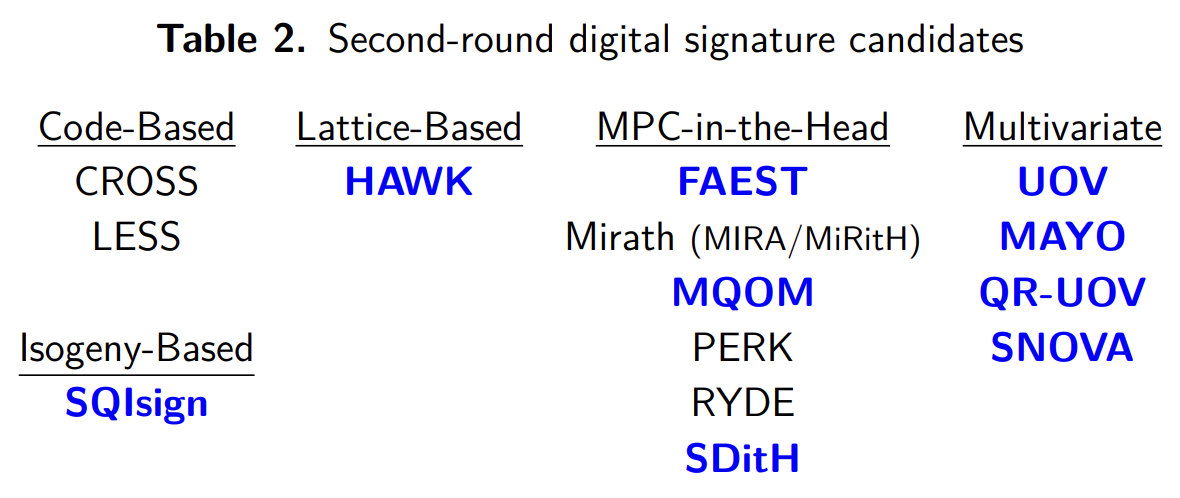
\includegraphics[width=0.6\linewidth]{figures/dsas.png}
    }
    \only<2->{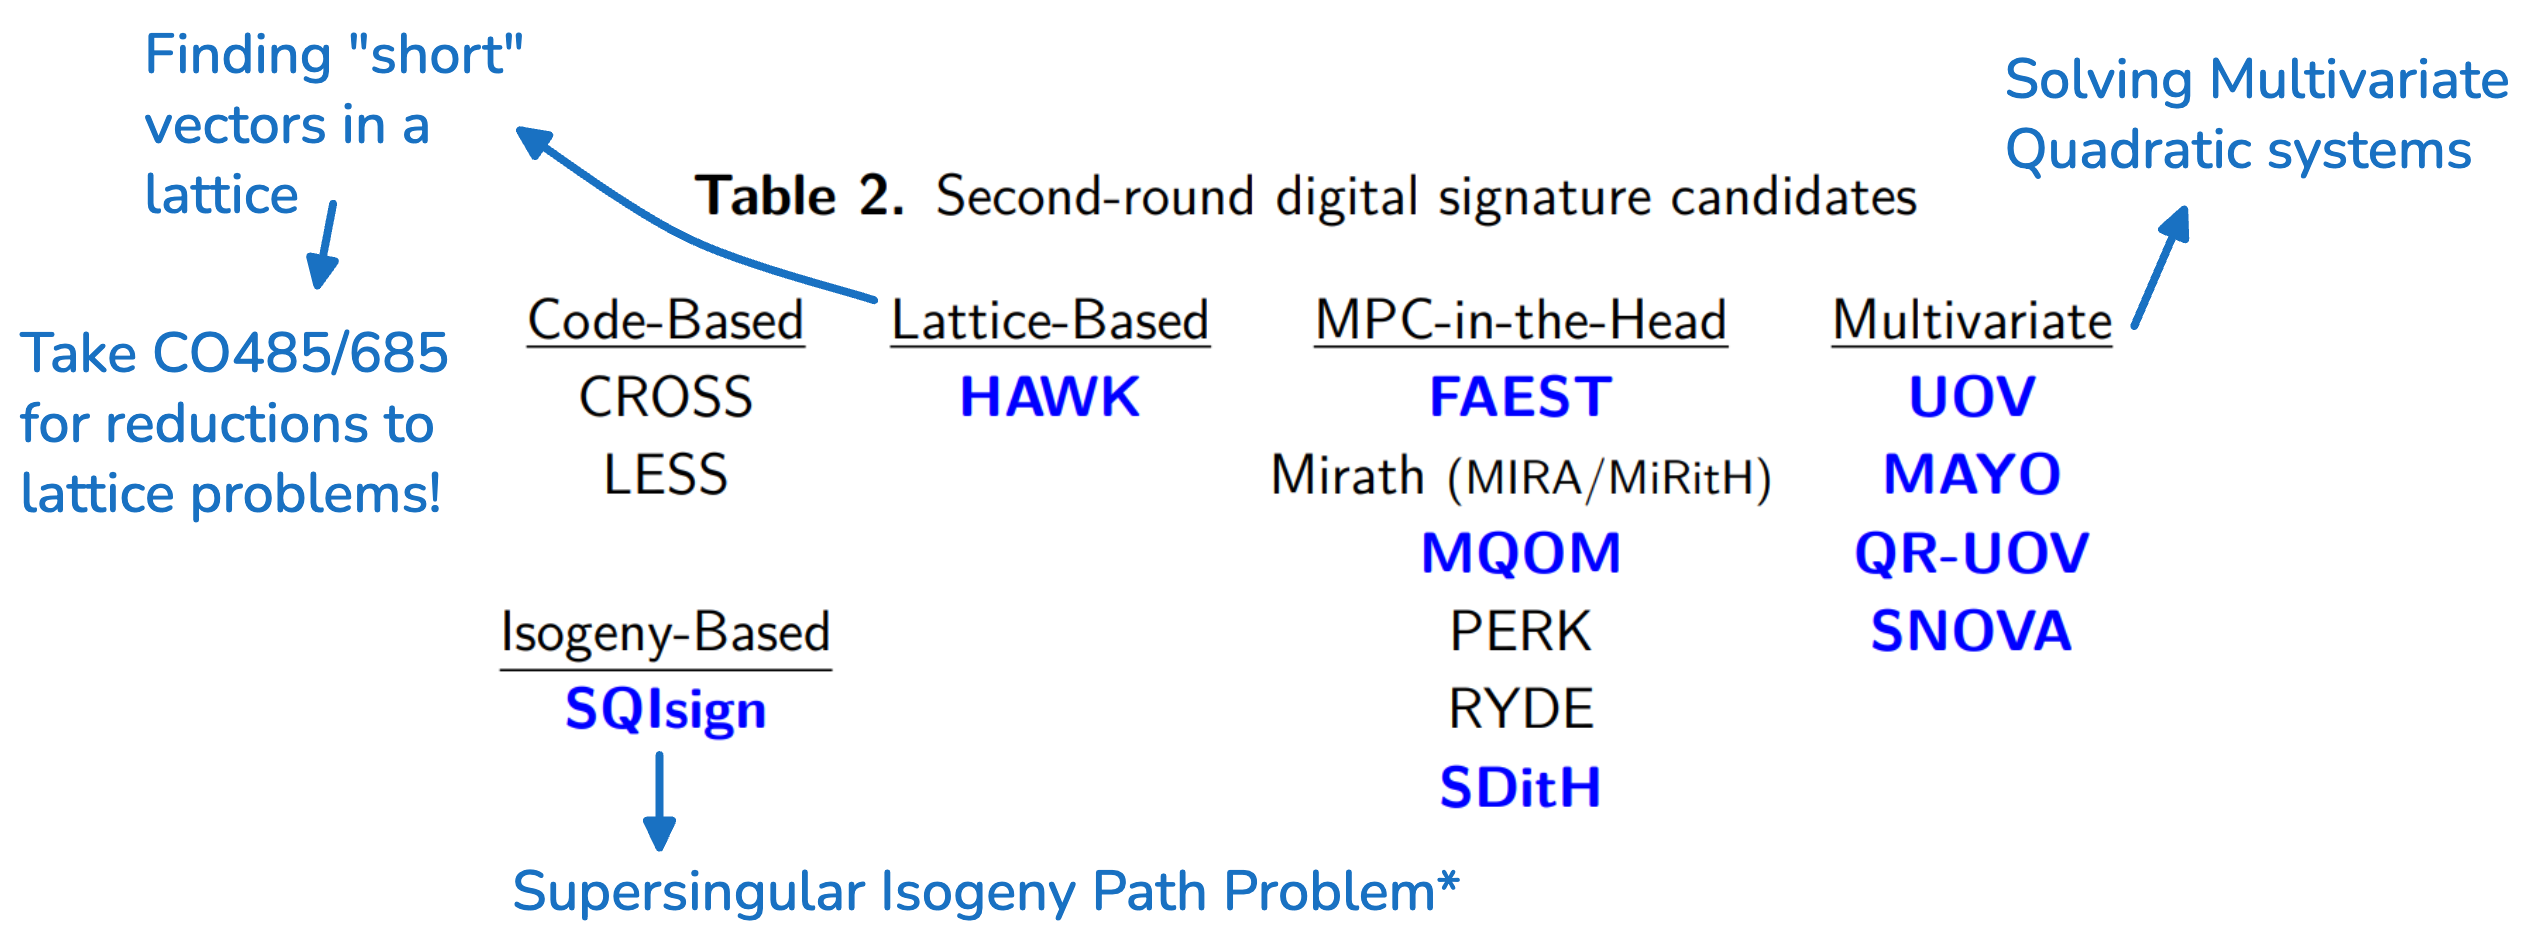
\includegraphics[width=0.9\linewidth]{figures/dsas_annotated.png}}
  \end{center}
\end{frame}

% ===== SECTION: THE OBJECTS =====
\section{Curves, isogenies, and a giant graph}

% ===== 5. CURVES AS DOTS ===== 
\begin{frame}{Elliptic curves: our vertex building blocks}
  \begin{columns}[T]
    \begin{column}{0.7\textwidth}
      Over a field, an elliptic curve is the set of points $(x,y)$ that satisfy
      \[ y^2 = x^3 + ax + b .\]
      along with a sentinel ``point at infinity''.
      \begin{itemize}
        \item We can define addition between two points.
        \item Using the ``point at infinity'' as an identity, this forms a \alert{group}!
        \item The \alert{$j$-invariant} is a fingerprint: it tells two curves apart up to isomorphism.
      \end{itemize}
    \end{column}
    \begin{column}{0.3\textwidth}
      \centering
      % --- Placeholder for the classic chord-and-tangent figure. ---
      % Drop in your own graphic, or sketch live on the board.
      \fbox{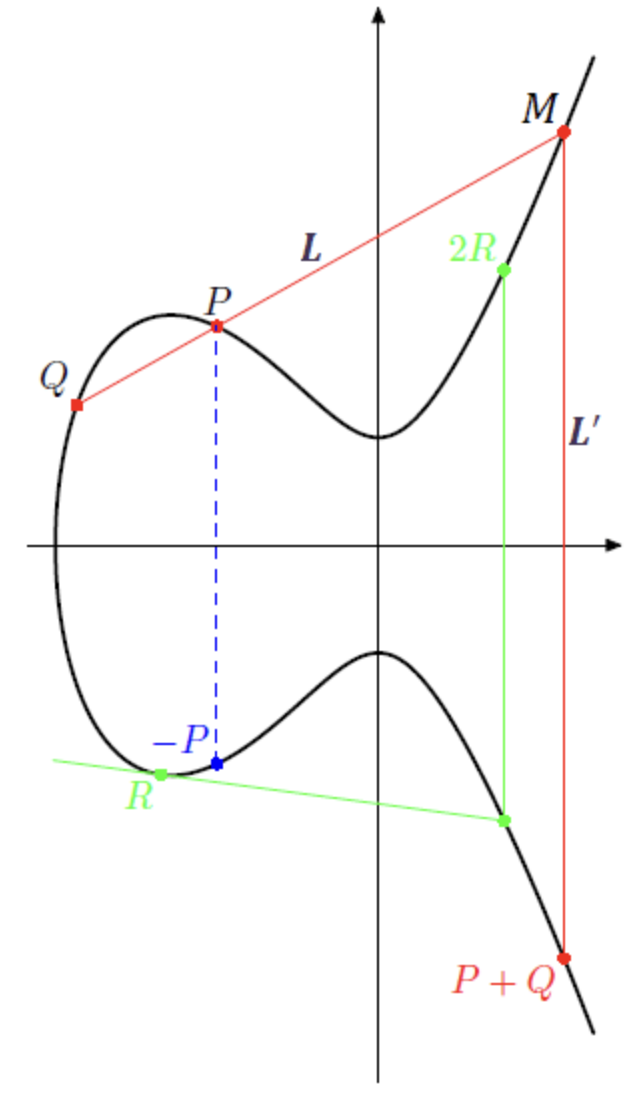
\includegraphics[width=0.8\linewidth]{figures/addition.png}}
    \end{column}
  \end{columns}
\end{frame}

\begin{frame}{Elliptic curves: our vertex building blocks}
  \begin{definition}[Elliptic curve]
    Over a field $\mathbb{F}_q$ with charactersitic $q \neq 2,3$, an \emph{elliptic curve} is the set of
    $(x,y)$ satisfying $y^2 = x^3 + ax + b$ with $4a^3 + 27b^2 \neq 0$, together with a point at
    infinity $\mathcal{O}$.
  \end{definition}
  \vspace{0.5em}
  \begin{theorem}[Group law]
    The points of $E$ form an abelian group under chord-and-tangent addition, with identity $\mathcal{O}$.
  \end{theorem}
  \vspace{0.5em}
  \begin{theorem}[Classification {\cite[III.1.4(b)]{silverman}}]
    Two elliptic curves are isomorphic over $\overline{\mathbb{F}}_p$ $\iff$ they share the same $j$-invariant,
    $j = 1728\,\dfrac{4a^3}{4a^3 + 27b^2}$.
  \end{theorem}
  For a comprehensive foundation of the math behind elliptic curves, take a look at \textit{The Arithmetic
of Elliptic Curves} (Silverman \cite{silverman})!
\end{frame}

% ===== 6. ISOGENIES AS ARROWS ===== 
\begin{frame}{Isogenies: our edges}
  Suppose $E_1,E_2$ are elliptic curves defined over $\mathbb{F}_q$. \\
  An \alert{isogeny} $\varphi: E_1 \to E_2$ is a non-constant rational map defined over $\mathbb{F}_q$ that is also a homomorphism.
  \begin{itemize}[<+(1)->]
    \item Preserves the group structure: if $P,Q\in E_1$ then $\varphi(P+Q) = \varphi(P)+\varphi(Q)$
    \item ``Being isogenous'' is an \textbf{equivalence relation} (there's always a dual isogeny).
    \item We say a seperable isogeny has \alert{degree} $\ell$ if it has a kernel of size $\ell$.
  \end{itemize}
  \vspace{0.8em}
  \centering
  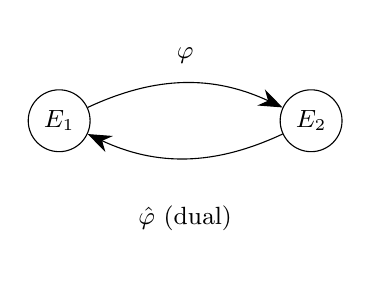
\begin{tikzpicture}[every node/.style={circle,draw,minimum size=7mm,font=\small}]
    \node (E1) {$E_1$};
    \node (E2) [right=2.4cm of E1] {$E_2$};
    \draw[-{Stealth[length=3mm]},bend left=25] (E1) to node[above,draw=none]{$\varphi$} (E2);
    \draw[-{Stealth[length=3mm]},bend left=25] (E2) to node[below,draw=none]{$\hat\varphi$ (dual)} (E1);
  \end{tikzpicture}
\end{frame}

\begin{frame}{Isogenies: our edges}
  \begin{definition}[Isogeny]
    An \emph{isogeny} $\varphi\colon E_1 \to E_2$ is a non-constant morphism defined over $\mathbb{F}_q$
    with $\varphi(\mathcal{O}) = \mathcal{O}$. Any such map is automatically a group homomorphism
    \cite[III.4.8]{silverman}.
  \end{definition}
  \vspace{0.5em}
  \begin{definition}[Degree {\cite[II.2]{silverman}}]
    The \emph{degree} of $\varphi$ is $\deg\varphi = [\,\overline{\mathbb{F}}_q(E_1) : \varphi^{*}\overline{\mathbb{F}}_q(E_2)]$.
    If $\varphi$ is separable, then $\deg\varphi = \#\ker\varphi$ \cite[~III.4.10]{silverman}.
  \end{definition}
  \vspace{0.5em}
  \begin{theorem}[Dual isogeny {\cite[III.6.1]{silverman}}]
    For every isogeny $\varphi$ of degree $m$ there is a unique \emph{dual} $\hat\varphi\colon E_2 \to E_1$
    with $\hat\varphi \circ \varphi = [m]$. In particular, being isogenous is an equivalence relation.
  \end{theorem}
  \vspace{0.5em}
\end{frame}


% ===== 8. WHY SUPERSINGULAR =====
\begin{frame}{Why \emph{Supersingular}?}
  Curves come in two types, distinguished by their endomorphism structure ($\text{End}(E)$ is the ring of isogenies of the form $E\to E$):
  \vspace{0.6em}
  \begin{itemize}[<+(1)->]
    \item \textbf{Ordinary:} \alert{commutative} symmetry. A quantum computer can take advantage of this extra strcuture (Childs--\alert{Jao}--Soukharev give a sub-exponential attack~\cite{cjs}).
    \item \textbf{Supersingular:} \alert{non-commutative}. No known shortcut without this structure.
  \end{itemize}
  \onslide<+(1)->{Also, there are some useful properties of supersingular curves that make things acutally computable.
  In particular, there are \alert{exactly $\ell+1$ isogenies of degree $\ell$} (counting multiplicities)
  originating from any supersingular curve $E$~\cite{sidh}.}
\end{frame}

\begin{frame}{Why \emph{Supersingular}?}
  \begin{definition}[Endomorphism Ring {\cite[III.4]{silverman}}]
    An \emph{endomorphism} of $E$ is an isogeny $E \to E$, together with the zero map. These form a
    ring $\text{End}(E)$ under pointwise addition and composition, always containing $\mathbb{Z}$ via
    the multiplication-by-$n$ maps $[n]$.
  \end{definition}
  % \vspace{0.5em}
  % \begin{definition}[Ordinary Elliptic Curves {\cite[III.9.4]{silverman}}]
  %   We say that an Elliptic curve $E$ is ordinary if $\text{End}(E)\cong\mathcal{O}$ where $\mathcal{O}$ is
  %   an order in an imaginary quadratic field (so $\text{End}(E)$ is \alert{commutative}).
  % \end{definition}
  \vspace{0.5em}
  \begin{definition}[Supersingular Elliptic Curves {\cite[V.3.1(a)]{silverman}}]
    We say that an Elliptic curve $E$ is supersingular if $\text{End}(E)\cong\mathcal{O}$ where $\mathcal{O}$ is
    an order in a quaternion algebra.
  \end{definition}
  \begin{theorem}[How many $\ell$-isogenies? {\cite{sidh}}]
    Supersingular curves are all defined over $\mathbb{F}_{p^2}$, and for every prime $\ell \neq p$ there are
    exactly \alert{$\ell+1$} isogenies of degree $\ell$ (counting multiplicities) originating from any
    given supersingular curve.
  \end{theorem}
\end{frame}

% ===== 7. BUILD THE GRAPH ===== 
\begin{frame}{Assemble the Isogeny Graph}
  \begin{itemize}[<+->]
    \item Fix a big prime $p$, and consider the supersingular elliptic curves over $\mathbb{F}_{p^2}$
    \item Vertices $\leftarrow$ elliptic curves of an isogeny class (isomorphic curves represent the same vertices)
    \item Edges $\leftarrow$ isogenies between two curves
  \end{itemize}
  \vspace{0.6em}
  \onslide<+->{
  \begin{alertblock}{Wait... isogenous is an equivalence relation}
    Isn't this one big, dense blob?
    \begin{center}
      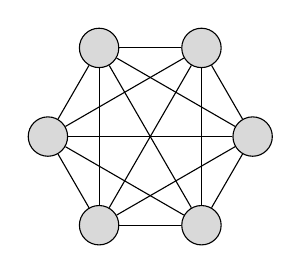
\begin{tikzpicture}[every node/.style={circle,draw,fill=black!15,minimum size=5mm,inner sep=0pt,font=\tiny}]
        \foreach \i in {0,1,2,3,4,5} {
          \node (n\i) at ({60*\i}:1.3cm) {};
        }
        % complete graph: connect every pair of vertices
        \foreach \i in {0,...,5} {
          \foreach \j in {0,...,5} {
            \ifnum\i<\j \draw (n\i)--(n\j); \fi
          }
        }
      \end{tikzpicture}
    \end{center}
  \end{alertblock}}
\end{frame}

\begin{frame}{Assemble the $\mathcolor{red}{\ell}$\textcolor{red}{-}Isogeny Graph}
  \begin{itemize}
    \item Fix a big prime $p$ \textcolor{red}{and a small prime} $\mathcolor{red}{\ell}$, and consider the supersingular elliptic curves over $\mathbb{F}_{p^2}$
    \item Vertices $\leftarrow$ elliptic curves of an isogeny class (isomorphic curves represent the same vertices)
    \item Edges $\leftarrow$ $\mathcolor{red}{\ell}$\textcolor{red}{-}isogenies between two curves
  \end{itemize}
  % bullets stay up from the start; +(1) offsets these reveals to clicks 2, 3, 4
  \onslide<+(1)->{Every vertex now has \alert{exactly} $\ell + 1$ neighbours.
  The result: an $(\ell+1)$-regular, connected, undirected graph.}
  \onslide<+(1)->{%
  \begin{center}
    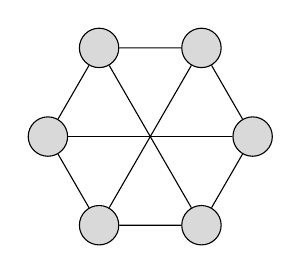
\begin{tikzpicture}[every node/.style={circle,draw,fill=black!15,minimum size=5mm,inner sep=0pt,font=\tiny}]
      \foreach \i in {0,1,2,3,4,5} {
        \node (n\i) at ({60*\i}:1.3cm) {};
      }
      % 3-regular (ell+1 = 3 for ell=2): hexagon cycle + the three long diagonals
      \draw (n0)--(n1)--(n2)--(n3)--(n4)--(n5)--(n0);
      \draw (n0)--(n3); \draw (n1)--(n4); \draw (n2)--(n5);
    \end{tikzpicture}
  \end{center}}
  \onslide<+(1)->{%
  \begin{alertblock}{The Supersingular Isogeny Path Problem (SIPP)}
    Given two supersingular curves $E_1, E_2$ over $\mathbb{F}_{p^2}$, find a \alert{path} between them
    in the $\ell$-isogeny graph. Equivalently, find an isogeny $E_1 \to E_2$ of degree $\ell^e$.
  \end{alertblock}}
\end{frame}


% ===== SECTION: HARDNESS =====
\section{Why is finding a path hard?}

% ===== 9. RAMANUJAN ===== 

\newcommand{\petersen}[4][]{%
  \begin{tikzpicture}[scale=1.15,
      vtx/.style={circle, draw=black!65, line width=0.7pt,
                  inner sep=0pt, minimum size=6mm},
      edg/.style={draw=black!45, line width=0.7pt}]
    \foreach \i in {0,...,4} {
      \coordinate (O\i) at ({90+72*\i}:2);
      \coordinate (I\i) at ({90+72*\i}:1);
    }
    \foreach \i in {0,...,4} {
      \pgfmathtruncatemacro{\j}{mod(\i+1,5)}
      \pgfmathtruncatemacro{\k}{mod(\i+2,5)}
      \draw[edg] (O\i) -- (O\j);   % outer pentagon
      \draw[edg] (O\i) -- (I\i);   % spokes
      \draw[edg] (I\i) -- (I\k);   % inner pentagram
    }
    \pgfmathsetmacro{\sa}{min(100,200*#2)}
    \pgfmathsetmacro{\sb}{min(100,200*#3)}
    \pgfmathsetmacro{\sc}{min(100,200*#4)}
    \foreach \v in {O1,O4,I0} { \node[vtx, fill=red!\sb!white] at (\v) {}; }
    \foreach \v in {O2,O3,I1,I2,I3,I4} { \node[vtx, fill=red!\sc!white] at (\v) {}; }
    \node[vtx, fill=red!\sa!white, #1] at (O0) {};
  \end{tikzpicture}%
}
\newcommand{\linf}{\max_i \bigl|p_t(i)-\pi(i)\bigr|}

\begin{frame}{Ramanujan graphs: sparse, yet impossibly well-connected}
  \begin{itemize}
    \item A \alert{Ramanujan graph} is an \emph{optimal expander}: few edges, yet everything is
          reachable in very few steps.
    \item Consequence: a \textbf{random walk mixes ridiculously fast}. After a handful of steps
          you're essentially \emph{uniformly anywhere}.
  \end{itemize}

  \begin{center}
    % Handout keeps only the final ($t=6$) state of the walk.
    \only<2|handout:0>{\petersen[very thick]{1}{0}{0}}%
    \only<3|handout:0>{\petersen[very thick]{0.5}{0.16667}{0}}%
    \only<4|handout:0>{\petersen[very thick]{0.33333}{0.16667}{0.02778}}%
    \only<5|handout:0>{\petersen[very thick]{0.25}{0.14815}{0.05093}}%
    \only<6|handout:0>{\petersen[very thick]{0.19907}{0.13272}{0.06713}}%
    \only<7|handout:0>{\petersen[very thick]{0.16590}{0.12191}{0.07806}}%
    \only<8>{\petersen[very thick]{0.14390}{0.11463}{0.08537}}%

    \medskip
    \only<2|handout:0>{$t=0$ \qquad $\linf = 0.900$}%
    \only<3|handout:0>{$t=1$ \qquad $\linf = 0.400$}%
    \only<4|handout:0>{$t=2$ \qquad $\linf = 0.233$}%
    \only<5|handout:0>{$t=3$ \qquad $\linf = 0.150$}%
    \only<6|handout:0>{$t=4$ \qquad $\linf = 0.099$}%
    \only<7|handout:0>{$t=5$ \qquad $\linf = 0.066$}%
    \only<8>{$t=6$ \qquad $\linf = 0.044$}%
  \end{center}

  \only<9>{
    \begin{alertblock}{The key theorem}
      The supersingular $\ell$-isogeny graph \textbf{is} a Ramanujan graph~\cite{pizer}.
    \end{alertblock}
  }
\end{frame}

\begin{frame}
  \begin{definition}[Ramanujan Graphs {\cite{lrs}}]
    Let $G = (\mathcal{V}, \mathcal{E})$ be a connected, finite $k$-regular graph on $h$ vertices,
    with adjacency matrix $A$, and let $\lambda_{\mathrm{triv}} = k$ denote the trivial
    eigenvalue afforded by the constant vectors. We say that $G$ is a
    \emph{Ramanujan graph} if every nontrivial eigenvalue $\lambda$ of $A$ with
    $\lambda \neq -k$ satisfies $|\lambda| \;\leq\; 2\sqrt{k-1}$.
  \end{definition}
  \begin{theorem}[Rapid Mixing {\cite{jmv}}]
    Let $G$ be a regular graph of degree $k$ on $h$ vertices. Suppose that the
    eigenvalue $\lambda$ of any nonconstant eigenvector satisfies the bound
    $|\lambda| \leq c$ for some $c < k$. Let $S$ be any subset of the vertices of $G$,
    and $x$ be any vertex in $G$. Then a random walk of length at least
    $
      \frac{\log 2h/|S|^{1/2}}{\log k/c}
    $
    starting from $x$ will land in $S$ with probability at least
    $\dfrac{|S|}{2h} = \dfrac{|S|}{2|G|}$.
  \end{theorem}
  \begin{theorem}[$\ell$-Isogeny Graph is Ramanujan {\cite{pizer}}]
    The supersingular $\ell$-isogeny graph \textbf{is} a Ramanujan graph.
  \end{theorem}
\end{frame}

% ===== 10. THE BACKROOMS (CLIMAX) =====  (12:45, ~2:30)
\begin{frame}{The isogeny backrooms}
  \begin{columns}[T]
    \begin{column}{0.6\textwidth}
      You wake up in a room. Somewhere out there is \emph{one specific door} you need.
      % +(1) holds click 1 for the scene-setting line alone
      \begin{itemize}[<+(1)->]
        \item There are $\sim 2^{256}\approx 10^{77}$ rooms.\\
              {\small (More than the $\sim\!10^{50}$ atoms in the Earth.)}
        \item Each room has only 3 or 4 doors.
        \item The graph mixes so well that running through random doors quickly leaves you \alert{uniformly anywhere}.
      \end{itemize}
      \vspace{0.5em}
      \onslide<+(1)->{Without a map, searching \emph{is} just this random wandering.\\[4pt]}
    \end{column}
    \begin{column}{0.38\textwidth}
      \centering
      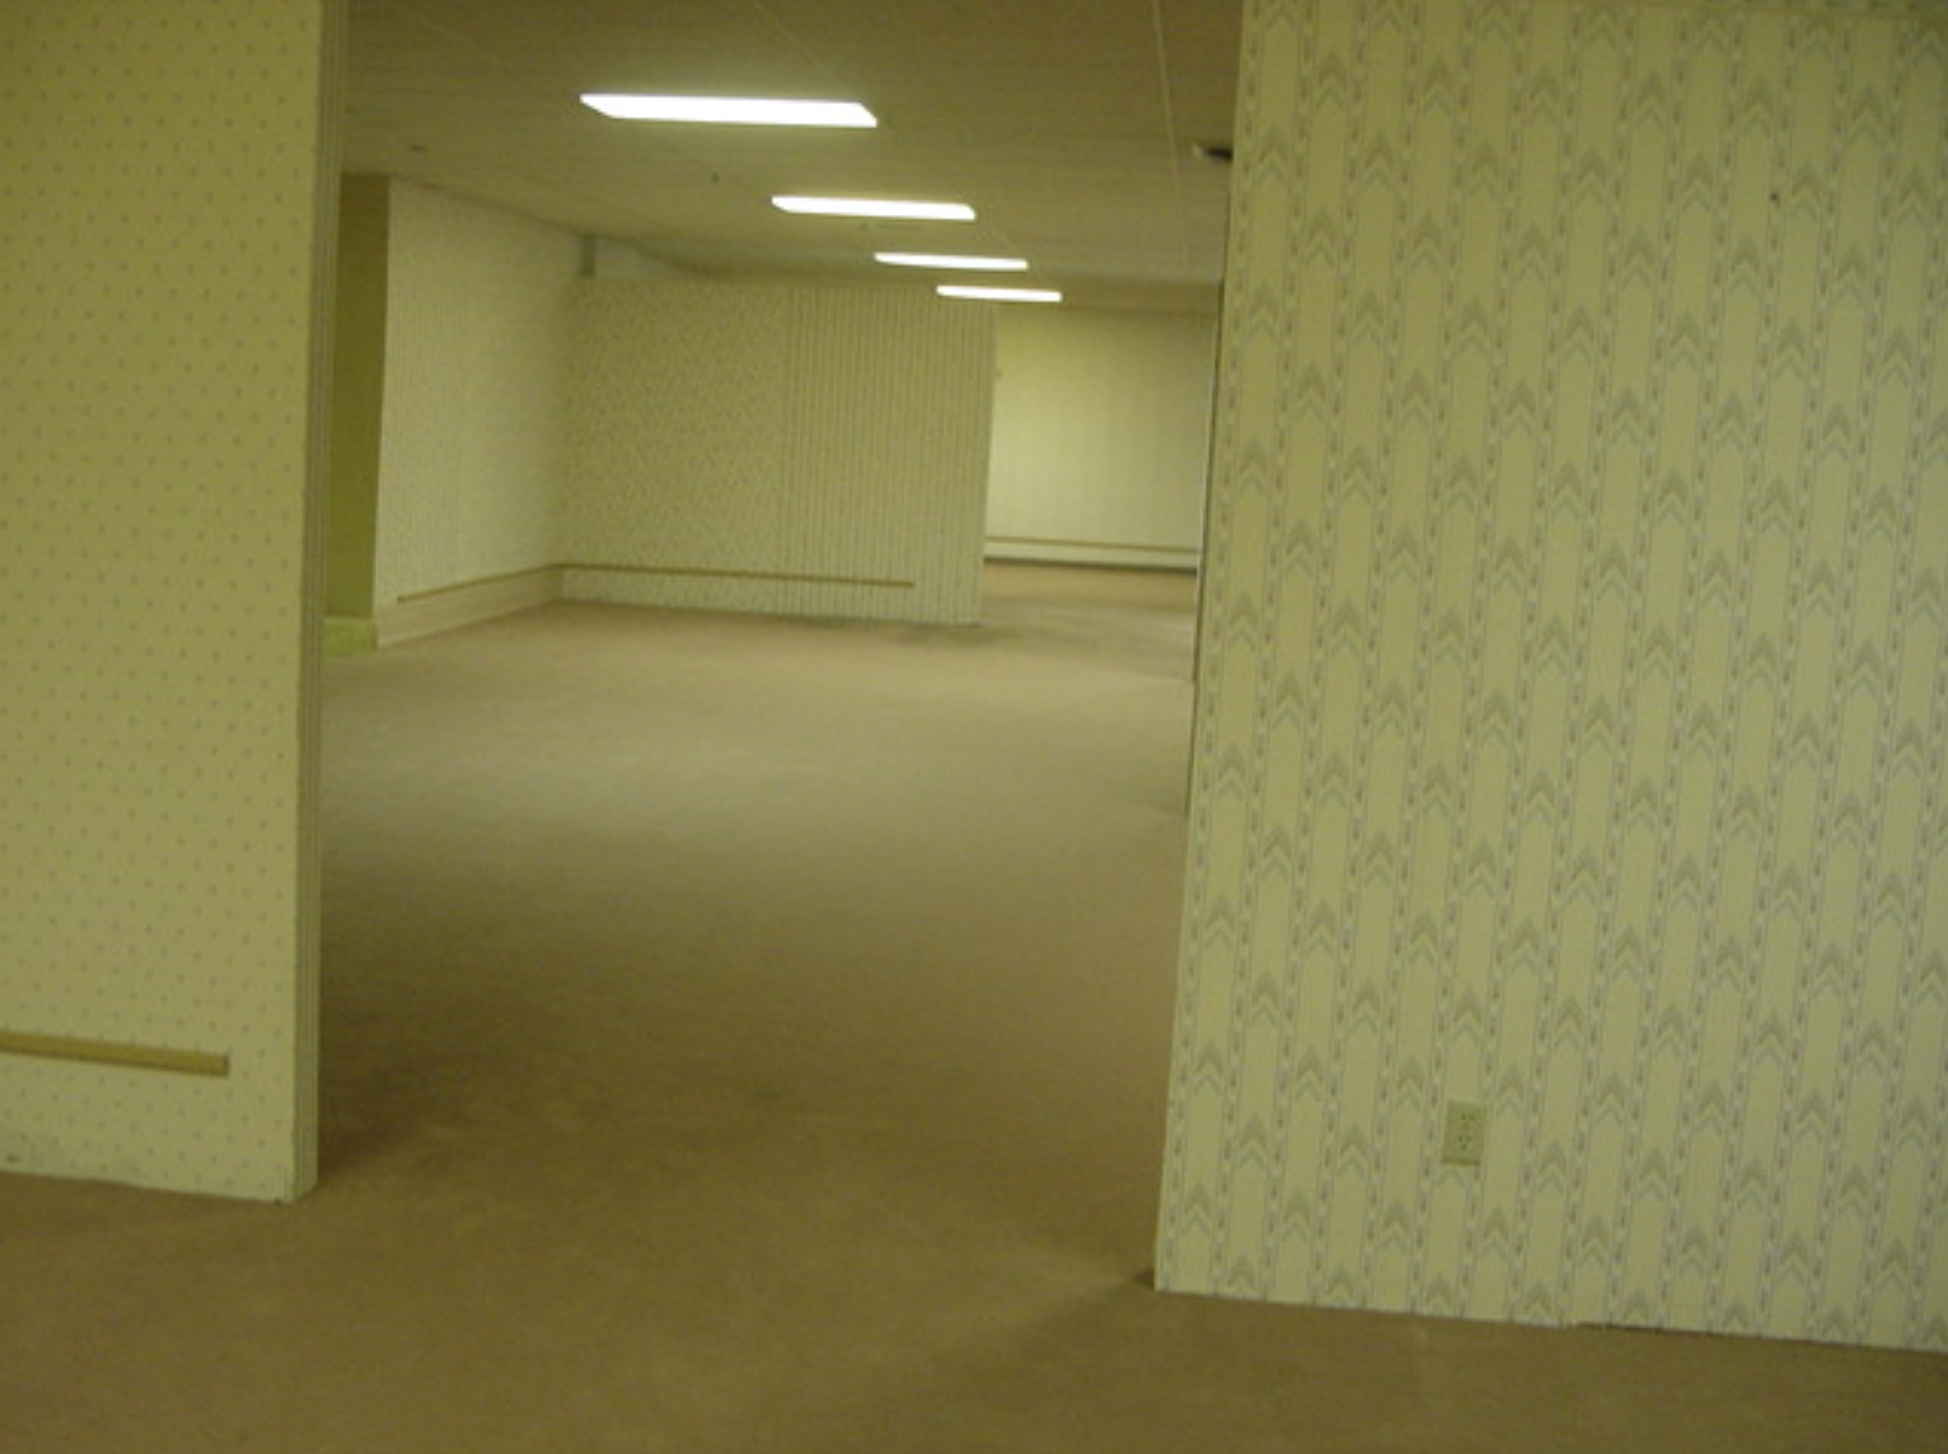
\includegraphics[width=0.9\linewidth]{figures/backrooms.png}
    \end{column}
  \end{columns}
\end{frame}

% ===== 11. WHAT REALLY MAKES IT HARD =====  (15:15, ~1:00)
\begin{frame}{But what \emph{really} makes it hard?}
  \onslide<+(1)->{
  Honestly? \alert{Our own inability.}}
  % +(1) holds click 1 for "Our own inability." alone
  \begin{itemize}[<+(1)->]
    \item \textbf{Even with a quantum computer} no fast attack is known. The best attacks
          stay exponential in the size of $p$.
    \item Its security really rests on the fact that nobody has cracked it \emph{yet}, despite having been investigated extensively by experts.
  \end{itemize}
  \vspace{0.6em}
  \centering\onslide<+(1)->{\alert{But... maybe you can solve it!}}
\end{frame}

% ===== SECTION: FROM PROBLEM TO SIGNATURE =====
\section{From a hard path to a signature}

% ===== 12. HARD PATH -> SIGNATURE =====  (16:15, ~2:00)
\begin{frame}{Our backdoor to the backrooms}
  The \alert{Deuring Correspondence}~\cite{deuring} turns our graph into a completely different object:
  a quaternion algebra.
  We can reason about these same ideas in this new language:
  % +(1) holds click 1 for the Deuring setup alone
  \begin{itemize}[<+(1)->]
    \item Each \textbf{curve} becomes a \alert{maximal order}: its endomorphism ring $\text{End}(E)$.
    \item Each \textbf{isogeny} becomes an \alert{ideal} joining two orders.
    \item The \textbf{degree} of an isogeny becomes the \alert{norm} of its ideal.
  \end{itemize}
  \vspace{0.8em}
  \onslide<+(1)->{In this new interpretation, an algorithm (\alert{KLPT}~\cite{klpt}) solves our path problem!}
  \onslide<+(1)->{The catch: computing $\text{End}(E)$ (what you need in order to translate) is itself
  \alert{as hard as finding a path}~\cite{wesolowski}.}

  \vspace{0.4em}
  \centering\onslide<+(1)->{But if you \emph{built} the curve yourself, you already know its endomorphism ring.
  \alert{This is our secret key!}}
\end{frame}

\begin{frame}{Our backdoor to the backrooms}
  \begin{theorem}[Deuring Correspondence {\cite{deuring}}]
    Let $B_{p,\infty}$ be the quaternion algebra over $\mathbb{Q}$ ramified exactly at $p$ and $\infty$.
    The map $E \mapsto \text{End}(E)$ is a bijection between supersingular curves over
    $\overline{\mathbb{F}}_p$ (up to Galois conjugacy) and maximal orders in $B_{p,\infty}$ (up to
    conjugation). Under it, an isogeny $\varphi: E_1 \to E_2$ corresponds to a left
    $\text{End}(E_1)$-ideal $I_\varphi$, with $\deg\varphi = \text{nrd}(I_\varphi)$ \cite[Ch.~42]{voight}.
  \end{theorem}
  \vspace{0.5em}
  \begin{theorem}[KLPT, 2014 {\cite{klpt}}]
    Given two maximal orders in $B_{p,\infty}$, there is a heuristically polynomial-time algorithm
    computing a connecting ideal of $\ell$-power norm. This translates to a \alert{path} in the $\ell$-isogeny graph.
  \end{theorem}
  So knowing $\text{End}(E_0)$ and $\text{End}(E_A)$ hands you the path $E_0 \to E_A$. The catch: recovering
  $\text{End}(E)$ from $E$ alone is itself as hard as finding a path.
\end{frame}

\begin{frame}{Two views of the same problem}
  \begin{center}
  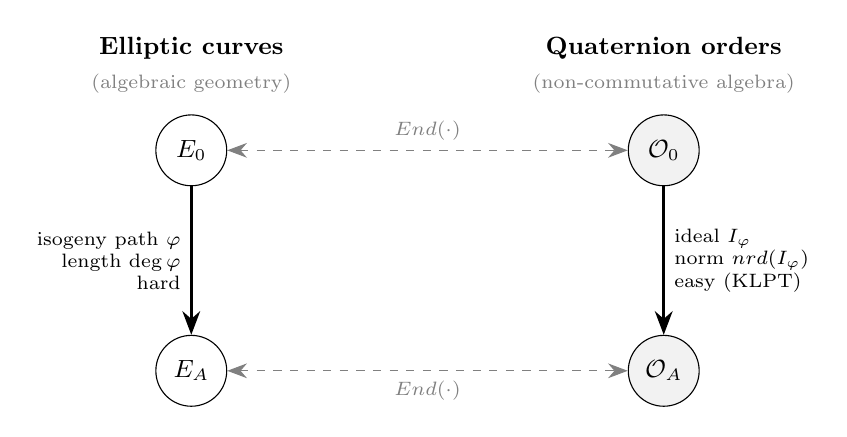
\begin{tikzpicture}[
      obj/.style={circle,draw,minimum size=9mm,font=\small},
      corr/.style={{Stealth[length=2.5mm]}-{Stealth[length=2.5mm]},dashed,gray},
      lbl/.style={font=\scriptsize}
    ]
    % --- headers (right-hand ones arrive with their column) ---
    \node[font=\bfseries\small] at (0,2.5)  {Elliptic curves};
    \node[lbl,gray]             at (0,2.05) {(algebraic geometry)};
    \node[font=\bfseries\small,visible on=<2->] at (6,2.5)  {Quaternion orders};
    \node[lbl,gray,visible on=<2->]            at (6,2.05) {(non-commutative algebra)};

    % --- 1. left: the geometry side ---
    \node[obj] (E0) at (0,1.2)  {$E_0$};
    \node[obj] (EA) at (0,-1.6) {$E_A$};
    \draw[-{Stealth[length=3mm]},line width=1pt]
      (E0) -- node[left,lbl,align=right]
        {isogeny path $\varphi$\\ length $\deg\varphi$\\ \alert{hard}} (EA);

    % --- 2. right: the algebra side ---
    \node[obj,fill=black!5,visible on=<2->] (O0) at (6,1.2)  {$\mathcal{O}_0$};
    \node[obj,fill=black!5,visible on=<2->] (OA) at (6,-1.6) {$\mathcal{O}_A$};
    \draw[visible on=<2->,-{Stealth[length=3mm]},line width=1pt]
      (O0) -- node[right,lbl,align=left,visible on=<2->]
        {ideal $I_\varphi$\\ norm $\text{nrd}(I_\varphi)$\\ \alert{easy (KLPT)}} (OA);

    % --- 3. the Deuring bridge ---
    \draw[corr,visible on=<3->] (E0) -- node[above,lbl,visible on=<3->] {$\text{End}(\cdot)$} (O0);
    \draw[corr,visible on=<3->] (EA) -- node[below,lbl,visible on=<3->] {$\text{End}(\cdot)$} (OA);
  \end{tikzpicture}
  \end{center}
  \centering\small Its the same problem in two languages. Crossing the dashed bridge needs
  $\text{End}(E)$ (which will be our secret).
\end{frame}


\begin{frame}{SQISign Step 1: Generate your keys}
  \begin{itemize}[<+->]
    \item Start with a public start curve $E_0$ where $\text{End}(E_0)$ is known
          (eg.\ $y^2 = x^3 + x$, which has $j = 1728$ and is supersingular when $p \equiv 3 \pmod 4$).
    \item Take a \alert{random walk} $\tau: E_0 \to E_A$ through the $\ell$-isogeny graph.
    \item Publish $E_A$ as your \alert{public key} 
    \item Conceal the path $\tau$ as your \alert{secret key}.
    \item Knowing $\tau$ also hands you $\mathcal{O}_A=\text{End}(E_A)$.
  \end{itemize}
  \vspace{0.4em}
  \begin{center}
  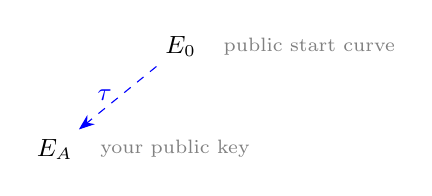
\begin{tikzpicture}[font=\small]
    % builds in step with the bullets: E_0 first, then the walk to E_A, then the key label
    \node (E0) at (1.6,1.3) {$E_0$};
    \node[visible on=<2->] (EA) at (0,0) {$E_A$};
    \draw[visible on=<2->,-{Stealth[length=2mm]},blue,dashed]
      (E0) -- node[left,pos=0.45,visible on=<2->] {$\tau$} (EA);
    \node[font=\scriptsize,gray,right=3pt of E0] {public start curve};
    \node[font=\scriptsize,gray,right=3pt of EA,visible on=<3->] {your public key};
  \end{tikzpicture}
  \end{center}
\end{frame}

\begin{frame}{SQISign Step 2: Come up with an interactive protocol}
  Prove you know $\text{End}(E_A)$ \emph{without revealing it}~\cite{sqisign}:
  \begin{enumerate}[<+->]
    \item \textbf{Commit}: walk a fresh random isogeny $\psi: E_0 \to E_1$, and publish $E_1$.
    \item \textbf{Challenge}: the verifier picks a random isogeny $\varphi: E_1 \to E_2$.
    \item \textbf{Response}: using $\mathcal{O}_A=\text{End}(E_A)$, produce an isogeny $\sigma: E_A \to E_2$.
    \item \textbf{Verify}: check $\sigma$ really is an isogeny $E_A \to E_2$ of the agreed degree.
  \end{enumerate}
  \vspace{0.2em}
  \begin{center}
  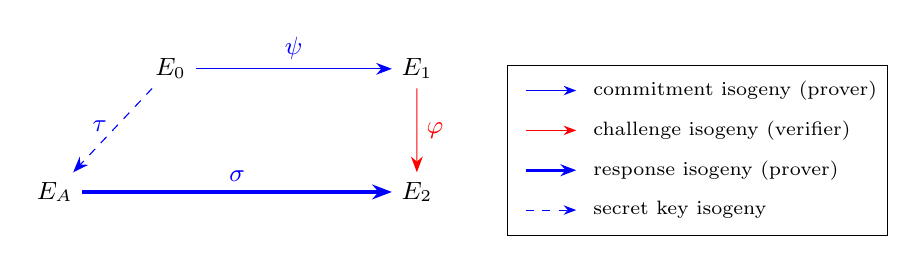
\begin{tikzpicture}[font=\small,scale=0.92]
    % --- the four curves (E_2 arrives with the challenge) ---
    \node (E0) at (1.6,1.7) {$E_0$};
    \node (E1) at (5.0,1.7) {$E_1$};
    \node (EA) at (0,0)     {$E_A$};
    \node[visible on=<2->] (E2) at (5.0,0)   {$E_2$};

    % --- the isogenies: each edge appears with its own bullet ---
    % setup carried over from Step 1: always visible
    \draw[-{Stealth[length=2mm]},blue,dashed] (E0) -- node[left,pos=0.45] {$\tau$} (EA);
    % 1. commit
    \draw[-{Stealth[length=2mm]},blue]        (E0) -- node[above] {$\psi$} (E1);
    % 2. challenge
    \draw[visible on=<2->,-{Stealth[length=2mm]},red]
      (E1) -- node[right,visible on=<2->] {$\varphi$} (E2);
    % 3. response
    \draw[visible on=<3->,-{Stealth[length=2.5mm]},blue,line width=1.2pt]
      (EA) -- node[above,visible on=<3->] {$\sigma$} (E2);

    % --- legend ---
    \begin{scope}[shift={(6.5,0)},font=\scriptsize]
      \draw[-{Stealth[length=1.6mm]},blue]        (0,1.4) -- (0.7,1.4);
      \node[right] at (0.8,1.4)  {commitment isogeny (prover)};
      \draw[-{Stealth[length=1.6mm]},red]         (0,0.85) -- (0.7,0.85);
      \node[right] at (0.8,0.85) {challenge isogeny (verifier)};
      \draw[-{Stealth[length=2mm]},blue,line width=1.2pt] (0,0.3) -- (0.7,0.3);
      \node[right] at (0.8,0.3)  {response isogeny (prover)};
      \draw[-{Stealth[length=1.6mm]},blue,dashed] (0,-0.25) -- (0.7,-0.25);
      \node[right] at (0.8,-0.25) {secret key isogeny};
      \draw (-0.25,-0.6) rectangle (5.0,1.75);
    \end{scope}
  \end{tikzpicture}
  \end{center}
  \vspace{-0.2em}
  \centering\small Reproduced from SQISign \cite[Fig.~1]{sqisign}.
\end{frame}

\begin{frame}{SQISign Step 3: Use the Fiat-Shamir transform to make the protocol non-interactive}
  The verifier's only real job was to provide an unpredictable challenge.
  \begin{itemize}
    \item So replace them with a hash: $\varphi = H(m \,\|\, E_1)$~\cite{fs}.
    \item A hash is unpredictable, so you still cannot cook up the challenge in advance.
    \item Binding the message $m$ into it makes the proof \alert{about that message}.
  \end{itemize}
  \vspace{0.8em}
  Your signature is the pair $(E_1, \sigma)$. Anyone recomputes $H(m \,\|\, E_1)$ and checks the
  response. All with no interaction required! \\
  \vspace{0.8em}
  For more on Fiat-Shamir transforms, take CO 485/684!
\end{frame}

% ===== 13. THE LINEAGE ===== 
\begin{frame}{The lineage of SQISign}
  \begin{itemize}
    \item \textbf{1941} --- \alert{Deuring}~\cite{deuring}: curves $\leftrightarrow$ quaternion orders.
    \item \textbf{1990} --- \alert{Pizer}~\cite{pizer}: the supersingular $\ell$-isogeny graph is Ramanujan.
    \item \textbf{2006} --- \alert{CGL} hash~\cite{cgl}: the isogeny-graph idea enters cryptography.
    \item \textbf{2011} --- \alert{SIDH}, by \alert{Jao \& De Feo, here at Waterloo}~\cite{sidh}: the first supersingular
          isogeny public-key scheme!
    \item \textbf{2014} --- \alert{KLPT}~\cite{klpt}: the quaternion side of the path problem falls...
    \item \textbf{2020} --- \alert{SQISign}~\cite{sqisign}: ...but Deuring $+$ KLPT gives a signature scheme!
    \item \textbf{2022} --- \alert{SIDH} is broken~\cite{cd}\ldots but because it leaked extra information.
          THe path problem itself survived.
    \item \textbf{2026} --- \alert{SQISign}~\cite{nistir8610}: one of nine schemes in NIST's Round 3, and the
          \emph{only} isogeny one still standing. \emph{(Last minute note: I learned they moved away from using KLPT by now...)}
  \end{itemize}
  \vspace{0.4em}
  \centering\small The idea was pioneered here, and it's still in the race!
\end{frame}

% ===== SECTION: WRAP =====
\section*{}

% ===== 14. RECAP =====  
\begin{frame}{Recap}
  \begin{enumerate}
    \item Curves are \alert{vertices}, $\ell$-isogenies are \alert{edeges}.
    \item The graph mixes so well that \alert{finding a path is hard} (Ramanujan $\to$ backrooms).
    \item That hardness \alert{builds digital signatures}.
  \end{enumerate}
  \vspace{0.8em}
  \centering{And it started right here at Waterloo!}
\end{frame}

% ===== 15. THANK YOU =====  (19:45)
\begin{frame}[plain]
  \centering
  \vfill
  {\Huge Thank you!}\\[0.6em]
  \large Questions?
  \vfill
\end{frame}
\note{
\textbf{19:45.} Done with ~15s of slack. Q\&A is a separate 5-minute block --- backup slides
follow.
}

% ============================================================
%  BACKUP SLIDES (after "Thank you", for predictable questions)
% ============================================================

% % ===== BACKUP A: WASN'T IT BROKEN? =====
% \begin{frame}{Backup: ``Wasn't isogeny crypto broken?''}
%   Yes-ish. \textbf{SIDH} was, in 2022 (Castryck--Decru~\cite{cd}).
%   \begin{itemize}
%     \item SIDH handed over \alert{extra torsion-point information} to make key exchange work.
%     \item That leak is what the attack exploited.
%     \item \textbf{SQISign doesn't reveal that information}, so it stands. The underlying
%           Supersingular Isogeny Path Problem was never solved.
%   \end{itemize}
% \end{frame}
% \note{Most likely question. Crisp answer + one more Waterloo-survivor flag.}

% % ===== BACKUP B: VERTEX COUNT =====
% \begin{frame}{Backup: how many vertices, exactly?}
%   Roughly $p/12$ supersingular $j$-invariants over $\overline{\mathbb{F}_p}$
%   (with small corrections depending on $p \bmod 12$).
%   \vspace{0.6em}

%   So ``$\sim 2^{256}$ rooms'' is the right \emph{order of magnitude} for a 256-bit prime ---
%   the constant out front doesn't change the backrooms.
% \end{frame}
% \note{For the stickler in row two.}

% ===== REFERENCES =====
\begin{frame}[allowframebreaks]{References}
  \small
  \begin{thebibliography}{8}
    \bibitem{silverman}
      J.~H. Silverman.
      \emph{The Arithmetic of Elliptic Curves}.
      2nd ed., GTM 106, Springer, 2009.
    \bibitem{lrs}
      Alexander Lubotzky, Ralph Phillips, and Peter Sarnak. 
      \emph{Ramanujan graphs}.
      Combinatorica, 8(3):261-277, 1988.
    \bibitem{jmv}
      David Jao, Stephen D. Miller, and Ramarathnam Venkatesan.
      \emph{Expander graphs based on GRH with an application to elliptic curve cryptography}. 
      J. Number Theory, 129(6):1491-1504, 2009.
    \bibitem{cgl}
      D.~X. Charles, K.~E. Lauter, E.~Z. Goren.
      \emph{Cryptographic hash functions from expander graphs}.
      Journal of Cryptology, 22(1):93--113, 2009.
    \bibitem{sidh}
      D.~Jao, L.~De~Feo.
      \emph{Towards quantum-resistant cryptosystems from supersingular elliptic curve isogenies}.
      PQCrypto 2011, LNCS 7071, 19--34.
    \bibitem{cjs}
      A.~Childs, D.~Jao, V.~Soukharev.
      \emph{Constructing elliptic curve isogenies in quantum subexponential time}.
      Journal of Mathematical Cryptology, 8(1):1--29, 2014.
    \bibitem{pizer}
      A.~K. Pizer.
      \emph{Ramanujan graphs and Hecke operators}.
      Bulletin of the AMS, 23(1):127--137, 1990.
    \bibitem{fs}
      A.~Fiat, A.~Shamir.
      \emph{How to prove yourself: practical solutions to identification and signature problems}.
      CRYPTO 1986, LNCS 263, 186--194.
    \bibitem{cd}
      W.~Castryck, T.~Decru.
      \emph{An efficient key recovery attack on SIDH}.
      EUROCRYPT 2023, LNCS 14008, 423--447.
    \bibitem{sqisign}
      L.~De~Feo, D.~Kohel, A.~Leroux, C.~Petit, B.~Wesolowski.
      \emph{SQISign: compact post-quantum signatures from quaternions and isogenies}.
      ASIACRYPT 2020, LNCS 12491, 64--93.
    \bibitem{deuring}
      M.~Deuring.
      \emph{Die Typen der Multiplikatorenringe elliptischer Funktionenk\"orper}.
      Abh. Math. Sem. Univ. Hamburg, 14:197--272, 1941.
    \bibitem{voight}
      J.~Voight.
      \emph{Quaternion Algebras}.
      GTM 288, Springer, 2021.
    \bibitem{klpt}
      D.~Kohel, K.~Lauter, C.~Petit, J.-P. Tignol.
      \emph{On the quaternion $\ell$-isogeny path problem}.
      LMS J. Comput. Math., 17(A):418--432, 2014.
    \bibitem{nistir8610}
      G.~Alagic et al.
      \emph{Status Report on the Second Round of the Additional Digital Signature Schemes for the
      NIST Post-Quantum Cryptography Standardization Process}.
      NIST IR 8610, May 2026. \texttt{doi:10.6028/NIST.IR.8610}
    \bibitem{ehlmp}
      K.~Eisentr\"ager, S.~Hallgren, K.~Lauter, T.~Morrison, C.~Petit.
      \emph{Supersingular isogeny graphs and endomorphism rings: reductions and solutions}.
      EUROCRYPT 2018, LNCS 10822, 329--368.
    \bibitem{wesolowski}
      B.~Wesolowski.
      \emph{The supersingular isogeny path and endomorphism ring problems are equivalent}.
      FOCS 2021, 1100--1111.
  \end{thebibliography}
\end{frame}

\end{document}
